\documentclass[border=3mm]{standalone}
\usepackage{fontspec,xeCJK,graphicx,tikz,amsmath}
\setmainfont{Helvetica}\setCJKmainfont{PingFang SC}
\usetikzlibrary{arrows.meta,positioning}
\definecolor{ink}{HTML}{173347}\definecolor{teal}{HTML}{217F83}\definecolor{amber}{HTML}{B96316}\definecolor{paper}{HTML}{FCFAF5}\definecolor{bluefill}{HTML}{EAF3F7}\definecolor{greenfill}{HTML}{E7F3EF}\definecolor{goldfill}{HTML}{FCEDDA}
\newsavebox{\sourcebox}\sbox{\sourcebox}{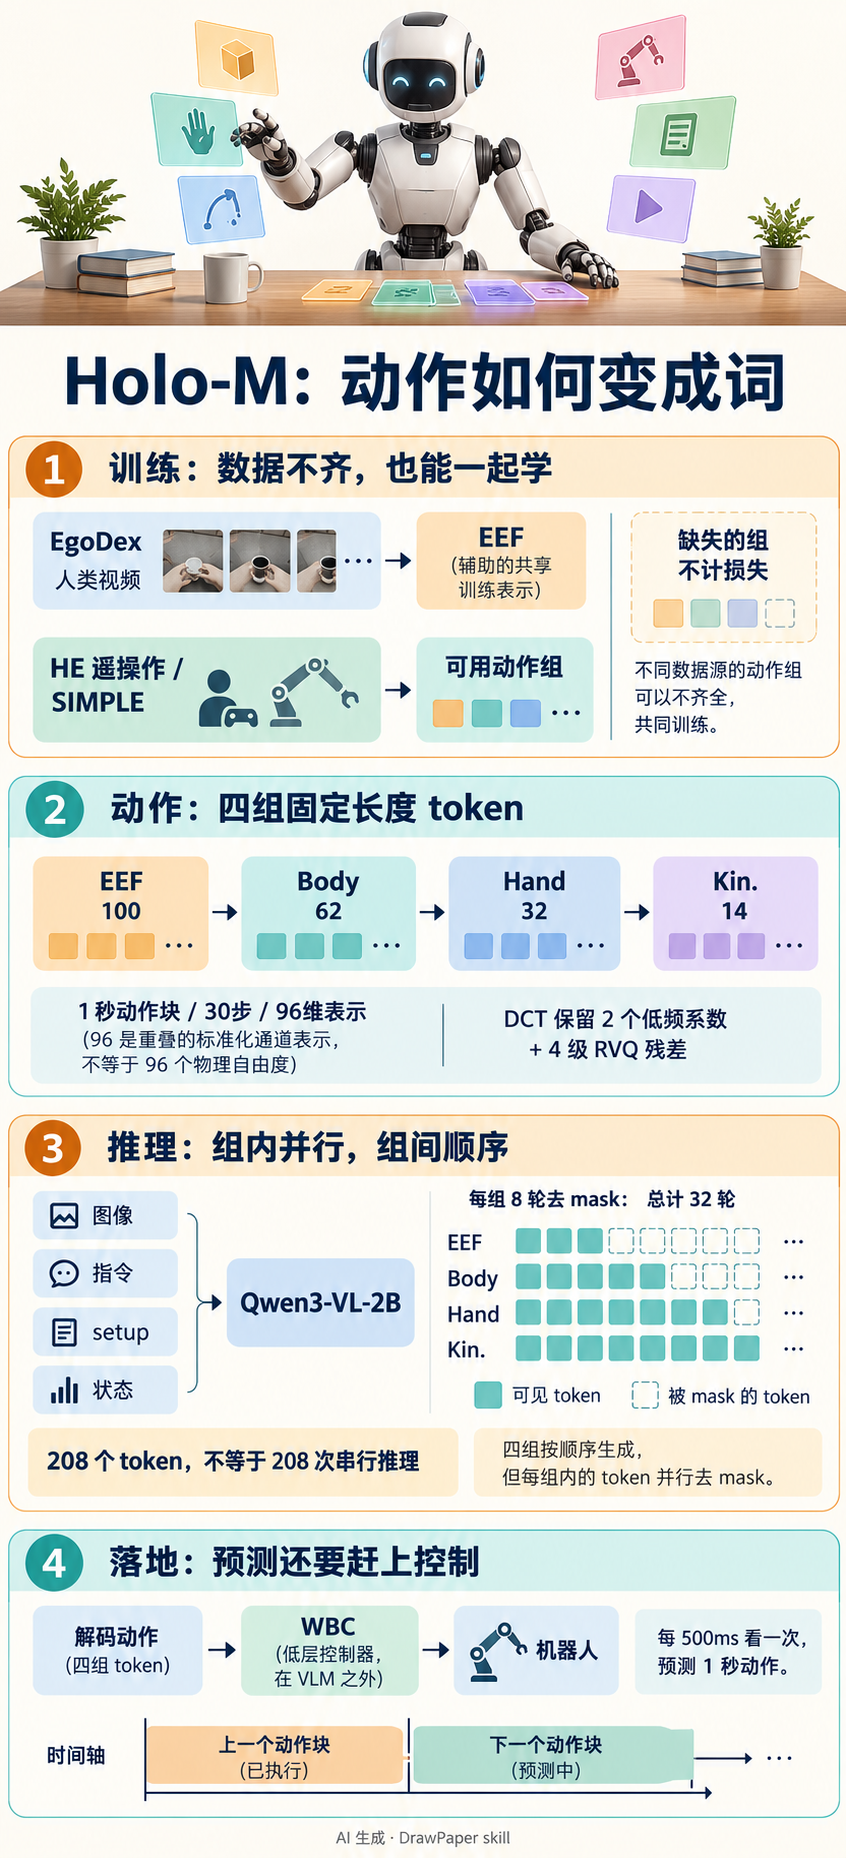
\includegraphics{holo-m-imagegen-draft.png}}
\newlength{\trimBottom}\setlength{\trimBottom}{.82455\ht\sourcebox}
\begin{document}
\begin{tikzpicture}[x=1cm,y=1cm,>=Latex,text=ink,txt/.style={align=center,font=\fontsize{16}{21}\selectfont},head/.style={align=left,font=\fontsize{19}{24}\selectfont\bfseries},box/.style={rounded corners=3mm,draw=teal!50,fill=bluefill,line width=.8pt},flow/.style={->,line width=1.4pt,draw=teal}]
\path[fill=paper] (-6.4,.2) rectangle (6.4,-33.4);
% Only conceptual illustration strip is retained; scientific labels are independently typeset.
\node[inner sep=0,anchor=north] at (0,0) {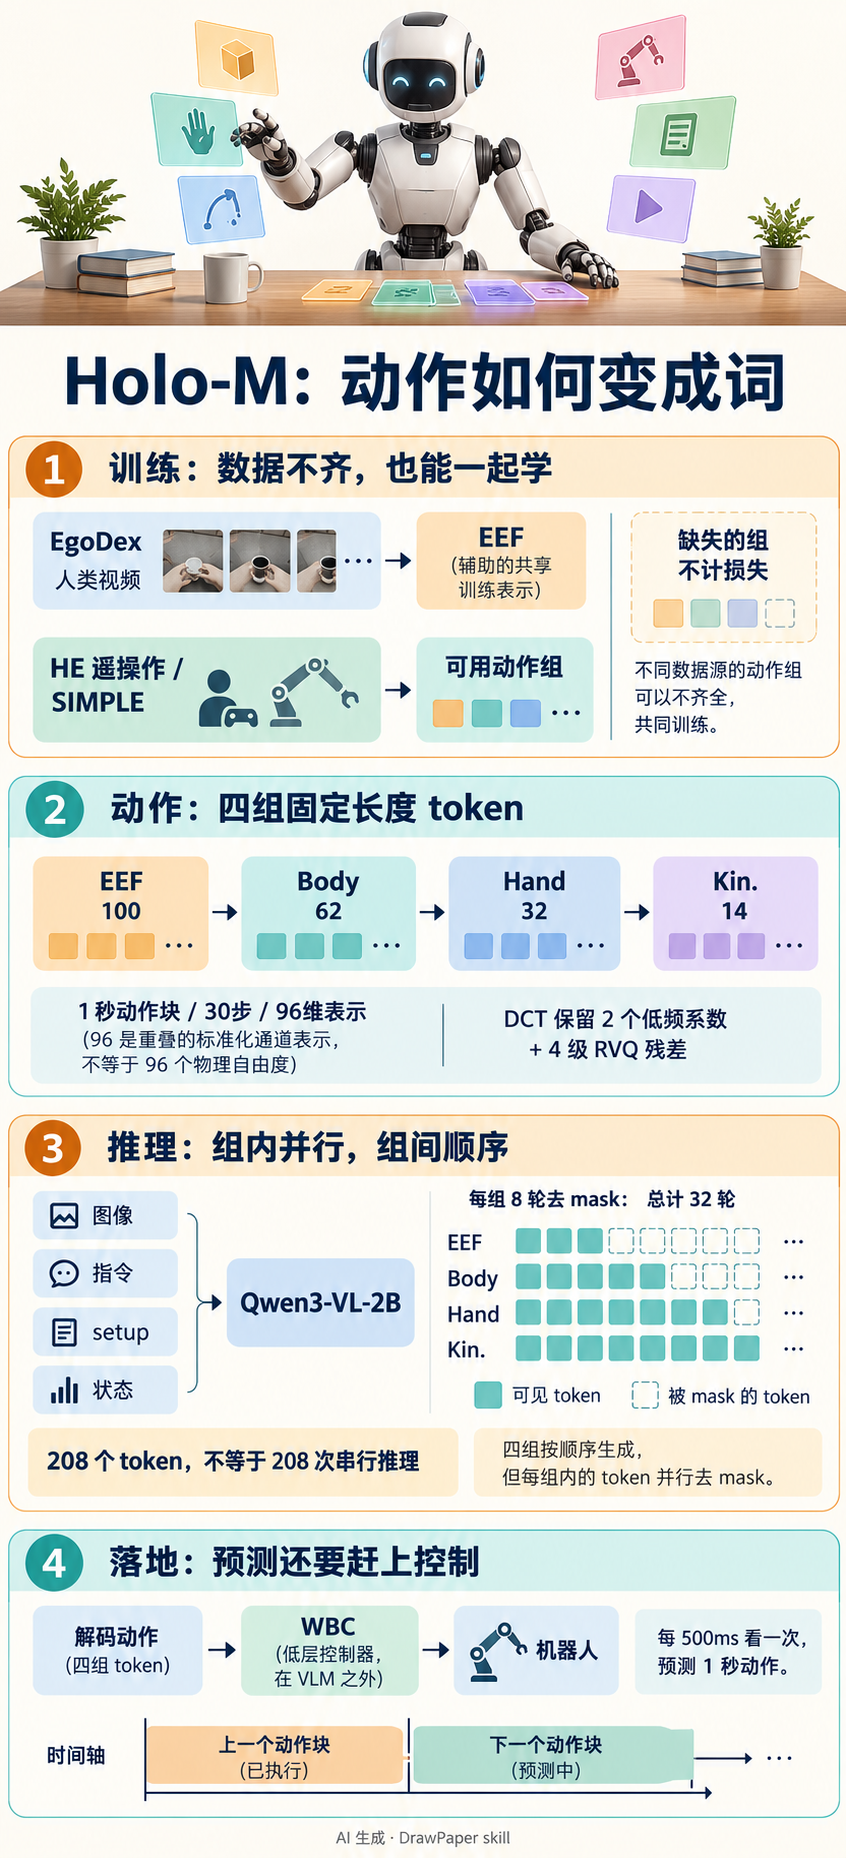
\includegraphics[viewport=0 1532 846 1858,clip,width=12.4cm]{holo-m-imagegen-draft.png}};
\node[head,align=center] at (0,-5.15) {Holo-M：动作如何变成词};
\node[txt,font=\fontsize{13}{17}\selectfont] at (0,-5.85) {概念机器人插画；不代表论文实机实验};
\draw[box,fill=goldfill,draw=amber!60] (-6.1,-6.35) rectangle (6.1,-10.55);
\node[head,anchor=west,text=amber] at (-5.8,-6.95) {1. 训练：只学数据里真的有的组};
\node[txt] at (0,-8.2) {EgoDex 人类视频：仅监督 EEF\\HE / SIMPLE：监督样本中可用的动作组};
\node[txt,font=\fontsize{15}{19}\selectfont] at (0,-9.7) {AR 预训练 $\to$ 人形对齐 $\to$ 去 mask 微调\\单任务适配可选；缺失组不计损失};
\draw[box] (-6.1,-10.9) rectangle (6.1,-16.4);
\node[head,anchor=west] at (-5.8,-11.5) {2. 表示：一秒动作，四组 token};
\foreach \xx/\lab/\num/\col in {-4.5/EEF/100/goldfill,-1.5/Body/62/greenfill,1.5/Hand/32/bluefill,4.5/Kin./14/goldfill}{\node[box,fill=\col,txt,minimum width=2.6cm,minimum height=1.2cm] at (\xx,-12.9) {\lab\\\num};}
\foreach \x in {-3,0,3}{\draw[flow] (\x-.15,-12.9)--(\x+.15,-12.9);}
\node[txt] at (0,-14.05) {30 步 × 96 维表示；96 不是电机数};
\node[txt,font=\fontsize{15}{20}\selectfont] at (0,-15.35) {每维 2 个 DCT 低频系数 + 4 级 RVQ\\$L_g=2D_g+4\quad\Rightarrow\quad L_{action}=208$};
\draw[box,fill=greenfill] (-6.1,-16.75) rectangle (6.1,-24.65);
\node[head,anchor=west,text=teal] at (-5.8,-17.4) {3. 生成：组内并行，组间顺序};
\node[box,fill=white,txt,minimum width=11cm,minimum height=1.6cm] (context) at (0,-18.75) {图像 + task + setup + 量化状态\\Qwen3-VL-2B（同一扩展词表）};
\node[box,fill=white,txt,minimum width=11cm,minimum height=1.6cm] (decode) at (0,-20.85) {EEF $\to$ Body $\to$ Hand $\to$ Kin.\\每组按置信度并行去 mask};
\draw[flow] (context.south)--(decode.north);
\foreach \xx in {-4.8,-3.6,-2.4,-1.2,0,1.2,2.4,3.6,4.8}{\draw[fill=teal!70,draw=teal!80,rounded corners=.8mm] (\xx-.35,-22.5) rectangle (\xx+.35,-22);}
\node[txt,font=\fontsize{15}{20}\selectfont] at (0,-23.2) {每组 8 轮 × 4 组 = 32 轮\\已完成组与条件前缀缓存};
\node[txt,font=\fontsize{15}{20}\selectfont] at (0,-24.2) {208 $\to$ 32 是顺序深度，不是实测加速倍数};
\draw[box,fill=goldfill,draw=amber!60] (-6.1,-25) rectangle (6.1,-32.4);
\node[head,anchor=west,text=amber] at (-5.8,-25.6) {4. 执行：模型还要赶上时钟};
\node[txt] at (0,-27.0) {解码为连续目标 $\to$ WBC $\to$ 机器人\\EEF 为共享训练表征；WBC 负责底层控制};
\node[txt,font=\fontsize{15}{19}\selectfont] at (0,-28.2) {每 500 ms 观测一次；预测 1 秒动作块};
% Concurrent execution and inference, not a measured duration plot.
\node[txt,font=\fontsize{14}{18}\selectfont,anchor=west] at (-5.65,-29.0) {同一时间窗：};
\node[box,fill=greenfill,txt,minimum width=8.5cm,minimum height=.65cm,anchor=west,font=\fontsize{15}{19}\selectfont] at (-2.9,-29.7) {执行上一动作块};
\node[box,fill=bluefill,txt,minimum width=8.5cm,minimum height=.65cm,anchor=west,font=\fontsize{15}{19}\selectfont] at (-2.9,-30.6) {推理下一动作块};
\node[txt,font=\fontsize{13}{17}\selectfont,align=left,anchor=west] at (-5.65,-30.15) {并行进行};
\node[txt,font=\fontsize{15}{19}\selectfont] at (0,-31.65) {后续新块丢弃 hold 内前段，再接管执行};
\node[txt,font=\fontsize{13}{17}\selectfont] at (0,-33.0) {AI 生成 · DrawPaper skill · 原文核对后的混合排版};
\end{tikzpicture}\end{document}
